\chapter{Anleitung}

\subsection{Bilder}

Einbindung eines Bildes:
\begin{figure}[ht]
	\begin{center}
		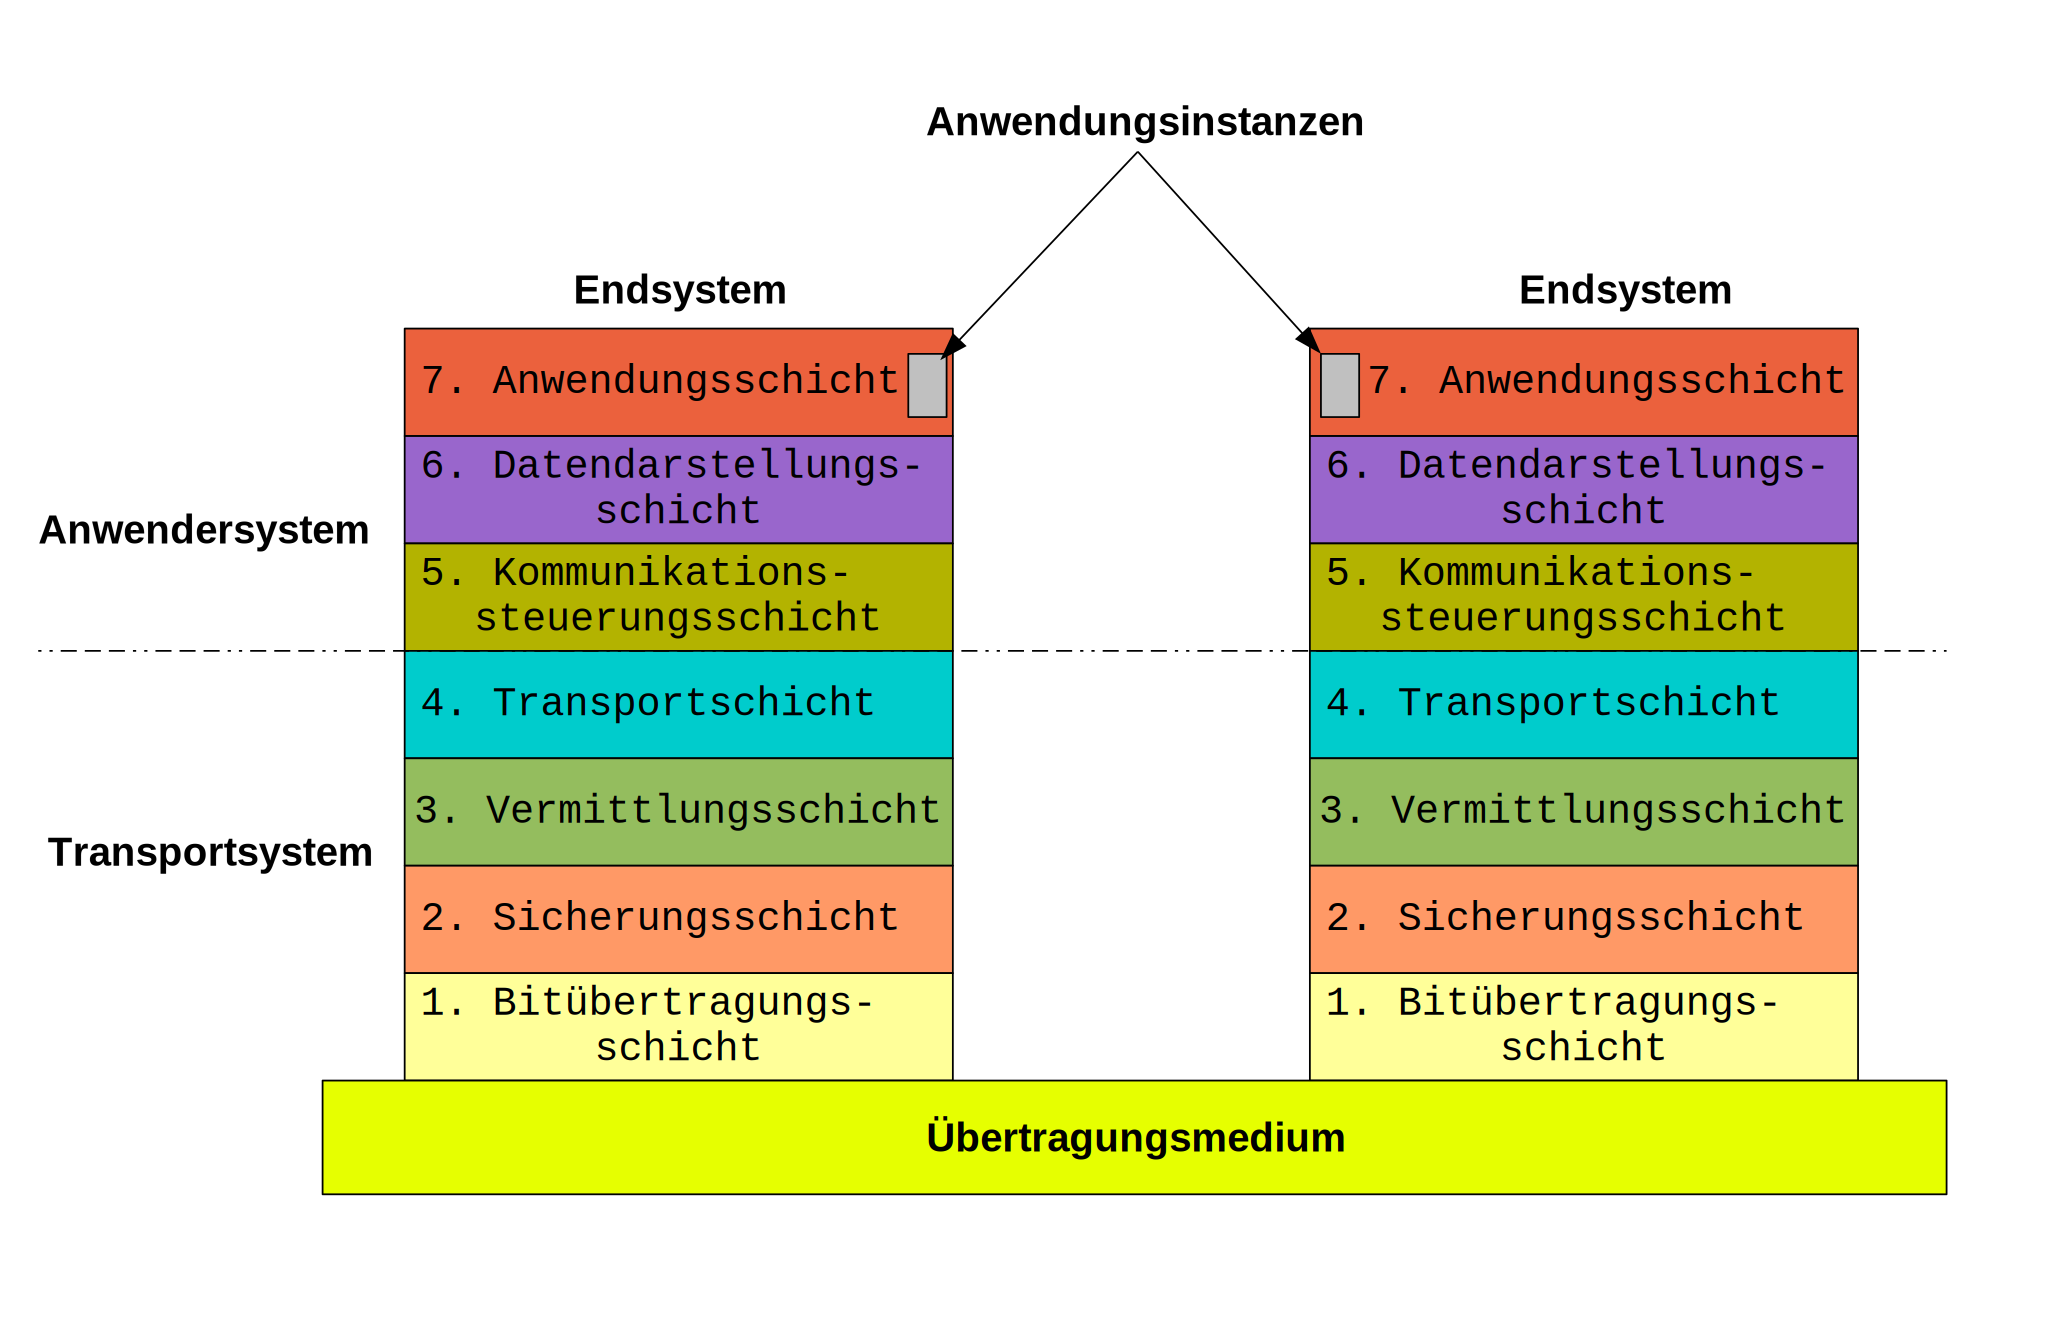
\includegraphics[width=0.9\textwidth]{./Bilder-Screenshots/ISO_OSI_Schichtenmodell.pdf}
		\caption{ISO OSI Schichtenmodell \cite{Deadlyhappen2014}}
		\label{OsiIsoModell}
	\end{center}
\end{figure}

Möchte man zwei bilder nebeneinander darstellen:
\begin{figure}[H]
	\centering
	\subfloat[][]{\includegraphics[width=0.4\linewidth]{./Bilder-Screenshots/Platzhalter}}
	\qquad
	\subfloat[][]{\includegraphics[width=0.4\linewidth]{./Bilder-Screenshots/Platzhalter}}

	\caption{a) Platzhalter1, b) Platzhalter2}
	\label{fig:ZweiBilder}
\end{figure}
\subsection{Listings}

\subsection{Inline}

\begin{listing}[ht]
	\caption{Python Test Code} 
	\label{lst:inlineCode}
	\begin{minted}[gobble=2] % entferne die Einrückung von x
		{python}
		print("hello, world")
	\end{minted}
\end{listing}


\subsection{Datei}

Um eine Datei einzubinden, die auf eine Seite passt:
\begin{listing}[H]
	\caption{Aufbau Initialisierungsdatei}
	\label{lst:aufbauInitialisierungsdatei}
	\inputminted[
	]{ini}
		{Listings/aufbau_initialisierungsdatei.ini}
\end{listing}

Um eine Datei einzubinden, die mehrere Seiten und somit einen Seitenumbruch benötigt:

\begingroup
	\captionsetup{type=listing}
	\inputminted[
		firstline=0,
		lastline=200
	]{python}
	{Listings/example.py}
	\captionof{listing}{Beispiel programm \label{lst:exampleCode}}
\endgroup


\subsection{Zitieren}

Ein sehr guter Vergleich was ein Hashwert ist wurde in \cite{SpringerKryptographie:2020} erbracht:
\begin{quotation}
	\quotes{
	Ein geeignetes mentales Modell für Hashfunktionen sind Fingerabdrücke
	von Personen. Es sollte praktisch unmöglich sein, zwei Personen zu finden, die exakt den
	gleichen Fingerabdruck haben, und aus einem Fingerabdruck kann man nicht die Person
	selbst rekonstruieren. Allerdings ist es einfach, einen Fingerabdruck zu bestimmen, wenn
	eine Person anwesend ist.
	}
\end{quotation}

\subsection{Acronyme}
Abkürzungen: \ac{VM}, \ac{SPS}

\subsection{TODOS}

\lipsum[11] \todo{Ein einfaches Todo}
\lipsum[11]

\todo[inline]{The original todo note withouth changed colours.\newline Here's another line.}
\lipsum[11]\unsure{Is this correct?}\unsure{I'm unsure about also!}
\lipsum[11]\change{Change this!}
\lipsum[11]\info{This can help me in chapter seven!}
\lipsum[11]\improvement{This really needs to be improved!\newline\newline What was I thinking?!}
\lipsum[11]
\thiswillnotshow{This is hidden since option `disable' is chosen!}
\improvement[inline]{The following section needs to be rewritten!}
\lipsum[11]
